\documentclass{article}\usepackage[]{graphicx}\usepackage[]{color}
%% maxwidth is the original width if it is less than linewidth
%% otherwise use linewidth (to make sure the graphics do not exceed the margin)
\makeatletter
\def\maxwidth{ %
  \ifdim\Gin@nat@width>\linewidth
    \linewidth
  \else
    \Gin@nat@width
  \fi
}
\makeatother

\definecolor{fgcolor}{rgb}{0.345, 0.345, 0.345}
\newcommand{\hlnum}[1]{\textcolor[rgb]{0.686,0.059,0.569}{#1}}%
\newcommand{\hlstr}[1]{\textcolor[rgb]{0.192,0.494,0.8}{#1}}%
\newcommand{\hlcom}[1]{\textcolor[rgb]{0.678,0.584,0.686}{\textit{#1}}}%
\newcommand{\hlopt}[1]{\textcolor[rgb]{0,0,0}{#1}}%
\newcommand{\hlstd}[1]{\textcolor[rgb]{0.345,0.345,0.345}{#1}}%
\newcommand{\hlkwa}[1]{\textcolor[rgb]{0.161,0.373,0.58}{\textbf{#1}}}%
\newcommand{\hlkwb}[1]{\textcolor[rgb]{0.69,0.353,0.396}{#1}}%
\newcommand{\hlkwc}[1]{\textcolor[rgb]{0.333,0.667,0.333}{#1}}%
\newcommand{\hlkwd}[1]{\textcolor[rgb]{0.737,0.353,0.396}{\textbf{#1}}}%

\usepackage{framed}
\makeatletter
\newenvironment{kframe}{%
 \def\at@end@of@kframe{}%
 \ifinner\ifhmode%
  \def\at@end@of@kframe{\end{minipage}}%
  \begin{minipage}{\columnwidth}%
 \fi\fi%
 \def\FrameCommand##1{\hskip\@totalleftmargin \hskip-\fboxsep
 \colorbox{shadecolor}{##1}\hskip-\fboxsep
     % There is no \\@totalrightmargin, so:
     \hskip-\linewidth \hskip-\@totalleftmargin \hskip\columnwidth}%
 \MakeFramed {\advance\hsize-\width
   \@totalleftmargin\z@ \linewidth\hsize
   \@setminipage}}%
 {\par\unskip\endMakeFramed%
 \at@end@of@kframe}
\makeatother

\definecolor{shadecolor}{rgb}{.97, .97, .97}
\definecolor{messagecolor}{rgb}{0, 0, 0}
\definecolor{warningcolor}{rgb}{1, 0, 1}
\definecolor{errorcolor}{rgb}{1, 0, 0}
\newenvironment{knitrout}{}{} % an empty environment to be redefined in TeX

\usepackage{alltt}
\usepackage{amsmath}
\usepackage{amssymb}
\IfFileExists{upquote.sty}{\usepackage{upquote}}{}
\begin{document}

% See excellent documentation at:
% http://yihui.name/knitr/
% http://yihui.name/knitr/demo/minimal/
% http://yihui.name/knitr/options
% ...as well as the manual knitr-manual.pdf, saved in this directory.





\title{Kernel Density Estimators}
\author{Timothy Meyers}
\maketitle

We will be exploring the performance of kernel estimators on the distribution shown in figure \ref{fig:plot_raw_data}.

\begin{knitrout}
\definecolor{shadecolor}{rgb}{0.969, 0.969, 0.969}\color{fgcolor}\begin{figure}[h!]


{\centering 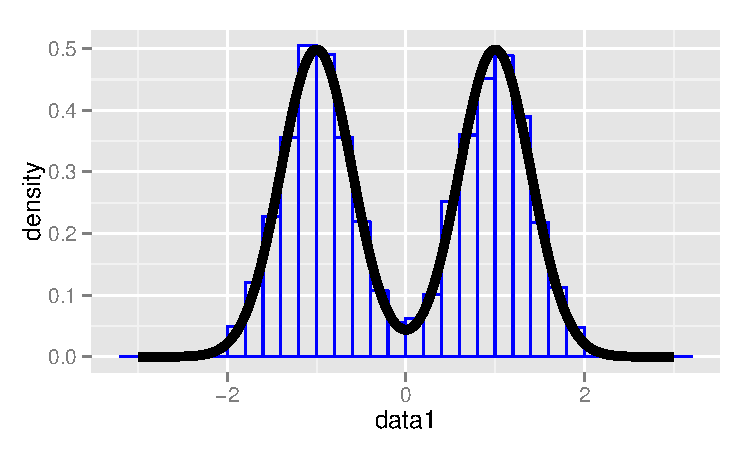
\includegraphics[width=\maxwidth]{figure/plot_raw_data} 

}

\caption[Raw data from a point mixture of normals]{Raw data from a point mixture of normals\label{fig:plot_raw_data}}
\end{figure}


\end{knitrout}

For all tasks, include a little text in this document about what you are doing.  When you're done, you'll have an R library and knitted pdf document.

TASK 1: Complete the Kernel function and plot it.

\ref{fig:plot_kernel}.
\begin{knitrout}
\definecolor{shadecolor}{rgb}{0.969, 0.969, 0.969}\color{fgcolor}\begin{figure}[h!]


{\centering 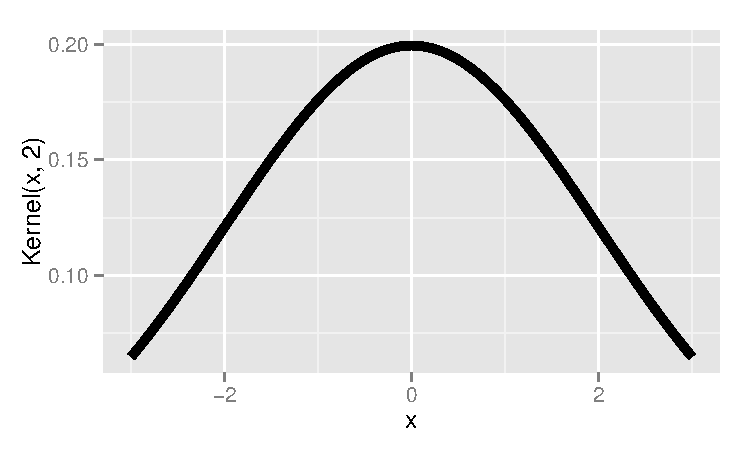
\includegraphics[width=\maxwidth]{figure/plot_kernel} 

}

\caption[Plotting the Kernel for a bunch of random points]{Plotting the Kernel for a bunch of random points\label{fig:plot_kernel}}
\end{figure}


\end{knitrout}

TASK 2: Complete the EstimateDensity function and try fitting it to your data with some different bandwidhts.

\ref{fig:plot_kernel_density}.
\begin{knitrout}
\definecolor{shadecolor}{rgb}{0.969, 0.969, 0.969}\color{fgcolor}\begin{kframe}


{\ttfamily\noindent\bfseries\color{errorcolor}{\#\# Error: Aesthetics must either be length one, or the same length as the dataProblems:EstimateDensity(x, Kernel, 2)}}\end{kframe}
\end{knitrout}

TASK 3: Complete the PerformSimulations function and make plots of the bias and variance.

TASK 4: Explore how the bias and variance changes as a function of the bandwidth.





\end{document}
